\documentclass[oneside, a4paper, 12pt]{book}

\usepackage[utf8x]{inputenc}   % omogoča uporabo slovenskih črk kodiranih v formatu UTF-8 
\usepackage[slovene,english]{babel}    % naloži, med drugim, slovenske delilne vzorce
\usepackage[pdftex]{graphicx}  % omogoča vlaganje slik različnih formatov 
\usepackage{fancyhdr}          % poskrbi, na primer, za glave strani
\usepackage{amssymb}           % dodatni simboli
\usepackage{amsmath}           % eqref, npr.


\renewcommand{\baselinestretch}{1.3} % ustrezen razmik med vrsticami



\newcommand{\BibTeX}{{\sc Bib}\TeX}

\newcommand{\autfont}{\Large}
\newcommand{\titfont}{\LARGE\bf}
\newcommand{\clearemptydoublepage}{\newpage{\pagestyle{empty}\cleardoublepage}}
\setcounter{tocdepth}{1}	      % globina kazala

% konstrukti
\newtheorem{izrek}{Izrek}[chapter]
%\newtheorem{trditev}{Trditev}[izrek]
\newenvironment{dokaz}{\emph{Dokaz.}\ }{\hspace{\fill}{$\Box$}}


\newcommand{\slika}[3]{
	\begin{figure}
	\begin{center}
	\includegraphics[keepaspectratio=true,width=9cm, height=9cm]{#1}
	\end{center}
	\vspace{-20pt}
	\caption{#2}
	\label{#3}
	\end{figure}
}


\begin{document}
\selectlanguage{slovene}
\frontmatter
\setcounter{page}{1} %
\renewcommand{\thepage}{}       % preprecimo težave s številkami strani v kazalu 

%%%%%%%%%%%%%%%%%%%%%%%%%%%%%%%%%%%%%%%%
%naslovnica
 \thispagestyle{empty}%
   \begin{center}
    {\large\sc Univerza v Ljubljani\\%
      Fakulteta za računalništvo in informatiko}%
    \vskip 10em%
    {\autfont Vojko Drev\par}%
    {\titfont Prenosni merilnik svetlobnih lastnosti žarometov \par}%
    {\vskip 2em \textsc{DIPLOMSKO DELO\\[2mm] 
	VISOKOŠOLSKEGA STROKOVNEGA ŠTUDIJA PRVE STOPNJE}\par}%
    \vfill\null%
    {\large \textsc{Mentor}: doc.\ dr.  Peter Peer\par}%
    {\vskip 2em \large Ljubljana, 2012 \par}%
\end{center}
% prazna stran
\clearemptydoublepage

%%%%%%%%%%%%%%%%%%%%%%%%%%%%%%%%%%%%%%%%
%copyright stran
\thispagestyle{empty}
\vspace*{8cm}
{\small \noindent
Rezultati diplomskega dela so intelektualna lastnina Fakultete za 
ra\-ču\-nal\-niš\-tvo in informatiko Univerze v Ljubljani. 
Za objavljanje ali izkoriščanje rezultatov di\-plom\-ske\-ga dela 
je potrebno pisno soglasje Fakultete za ra\-ču\-nal\-niš\-tvo in 
informatiko ter mentorja.}

% prazna stran
\clearemptydoublepage

%%%%%%%%%%%%%%%%%%%%%%%%%%%%%%%%%%%%%%%%
% stran 3 med uvodnimi listi
\noindent
%Namesto te strani {\bf vstavite} original izdane teme diplomskega 
%dela s podpisom mentorja in dekana ter žigom fakultete, ki ga diplomant
%dvigne v študent\-skem referatu,  preden odda izdelek v vezavo!
%Glej tudi sam konec Poglavja~\ref{ch2} na strani~\pageref{pp}.

\begin{figure}
\begin{center}
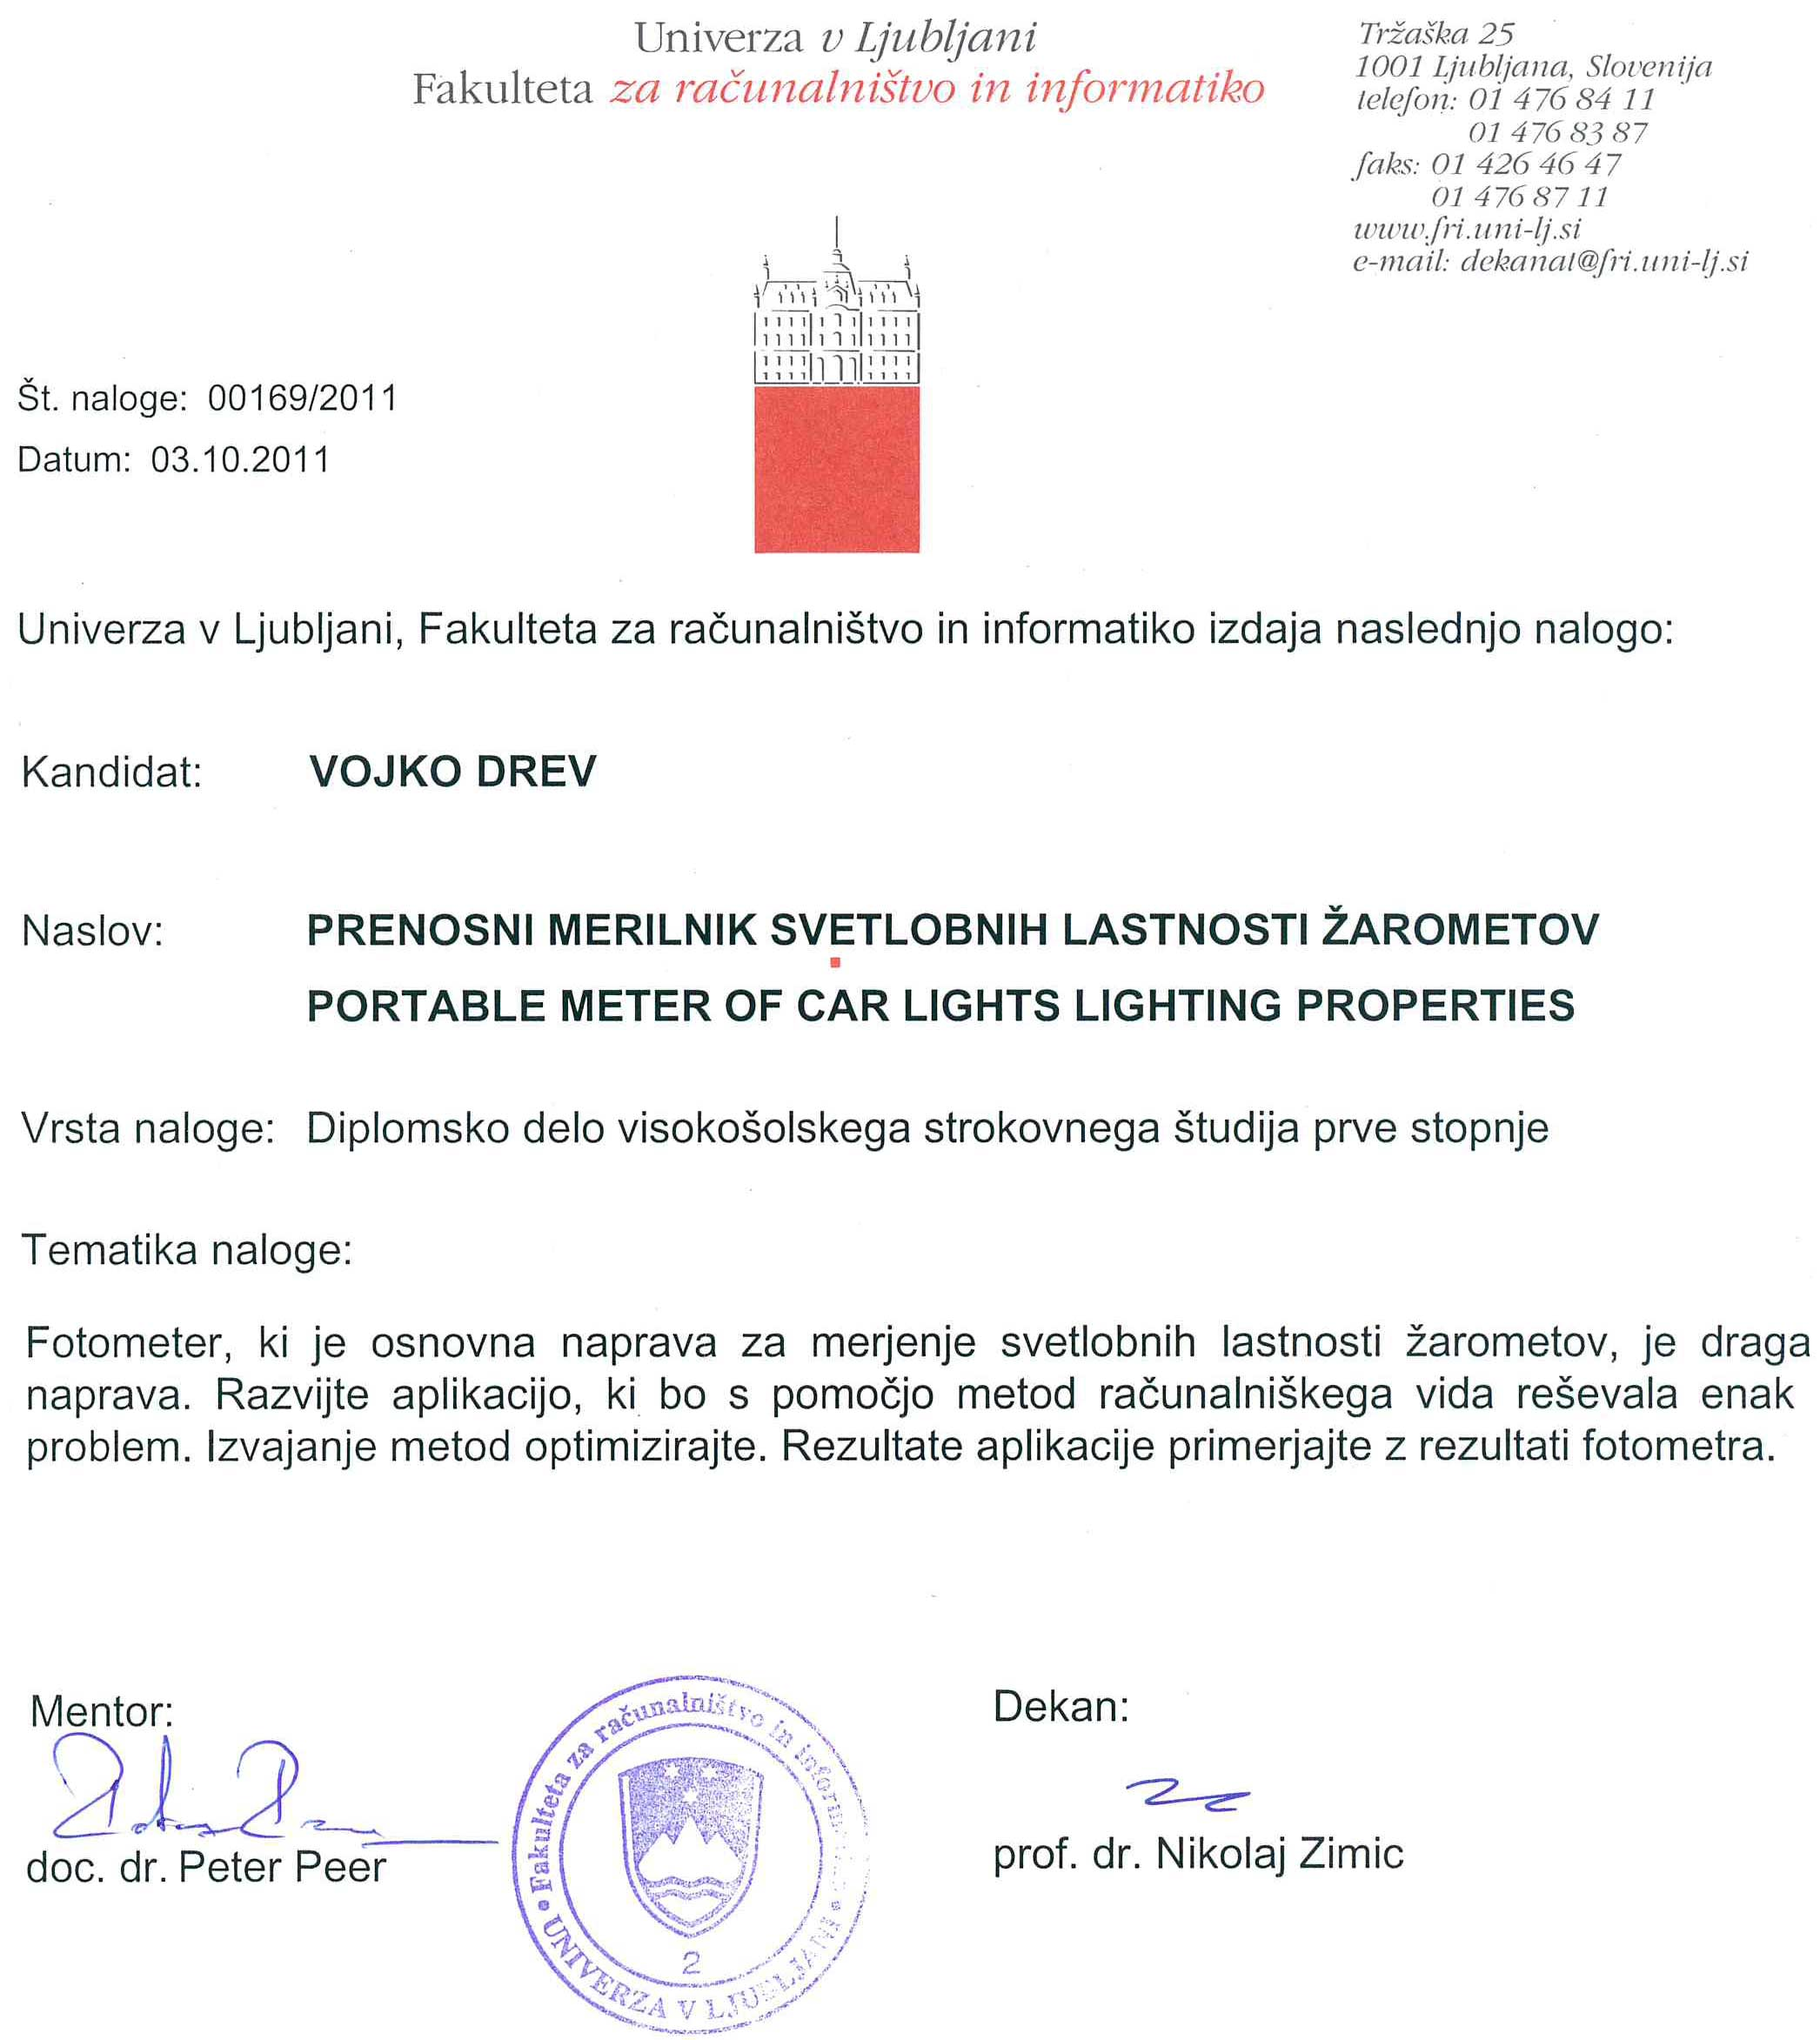
\includegraphics[keepaspectratio=true, width=13.5cm]{slike/original-teme.jpg}
\end{center}
\end{figure}

% prazna stran
\clearemptydoublepage

%%%%%%%%%%%%%%%%%%%%%%%%%%%%%%%%%%%%%%%%
% izjava o avtorstvu
\vspace*{1cm}
\begin{center} 
{\Large \textbf{\sc Izjava o avtorstvu diplomskega dela}}
\end{center}

\vspace{1cm}
\noindent Vojko Drev,
z vpisno številko \textbf{63050026}, sem avtor  diplomskega dela z 
naslovom:
   
\vspace{0.5cm}
\emph{Prenosni merilnik svetlobnih lastnosti žarometov.}

\vspace{1.5cm}
\noindent S svojim podpisom zagotavljam, da:
\begin{itemize}
	\item sem diplomsko delo izdelal samostojno pod mentorstvom 
		doc.\ dr.\ Petra Peera,

	\item	so elektronska oblika diplomskega dela, naslov (slov., angl.), 
	povzetek (slov., angl.) ter ključne besede (slov., angl.) identični s 
	tiskano obliko diplomskega dela in
	\item soglašam z javno objavo elektronske oblike diplomskega dela 
	v zbirki ''Dela FRI''.
\end{itemize}

\vspace{1cm}
\noindent V Ljubljani, dne 15. aprila 2012 \hfill Podpis avtorja:
\begin{figure}[h]
\hfill
\includegraphics[keepaspectratio=true,width=4cm]{slike/podpis.JPG}
\end{figure}


% prazna stran
\clearemptydoublepage

%%%%%%%%%%%%%%%%%%%%%%%%%%%%%%%%%%%%%%%%
% zahvala
\thispagestyle{empty}\mbox{}\vfill\null\it%
Zahvaljujem se mentorju doc. dr. Petru Peer, za pomoč in svetovanje pri 
izdelavi diplomske naloge.

Zahvaljujem se tudi mag. Janku Kerncu in podjetju Hella Saturnus 
Slovenija d.o.o., ki sta mi omogočila material, izvedbo in testiranje 
za diplomsko delo.

Hvaležen sem mojim staršem, prijateljem in vsem, ki so me podpirali in 
spodbujali pri študiju.
\rm\normalfont

% prazna stran
\clearemptydoublepage

%%%%%%%%%%%%%%%%%%%%%%%%%%%%%%%%%%%%%%%%
% posvetilo
\thispagestyle{empty}\mbox{}{\vskip0.20\textheight}\mbox{}\hfill\begin{minipage}{0.90\textwidth}%
\begin{flushright}
If I have seen further it is by standing on the shoulders of giants.\\
\textbf{Isaac Newton}
\end{flushright}
\normalfont\end{minipage}
 
% prazna stran
\clearemptydoublepage

%%%%%%%%%%%%%%%%%%%%%%%%%%%%%%%%%%%%%%%%
% kazalo
\def\thepage{}% preprecimo tezave s stevilkami strani v kazalu 
\tableofcontents{}


% prazna stran
\clearemptydoublepage

%%%%%%%%%%%%%%%%%%%%%%%%%%%%%%%%%%%%%%%%
% povzetek 
\addcontentsline{toc}{chapter}{Povzetek}
\chapter*{Povzetek}
\chaptermark{}
Cilj diplomske naloge je razviti program za preverjanje svetilnih 
lastnosti avtomobilskih žarometov. Vhodni parameter programa je slika 
snopa svetlobe žarometa. Ta sveti na steno (zaslon), kjer so narisane 
vodilne črte. Tri horizontalne in ena vertikalna. Žaromet se postavi 
tako, da sveti pravokotno na centralno vertikalno in horizontalno črto. 
Program iz slike izračuna prehod svetlo-temne meje po celotni širini 
slike. Uporabnik lahko izbere posamezno vertikalo. Njene intenzitete 
svetlobe se nato prikažejo na grafu. Vmesnik je zasnovan na principu 
vtičnikov. Te se preberejo iz določene mape na disku in naložijo v 
program dinamično. Vsak v svoj zavihek. Za komuniciranje med sabo 
uporabljajo model založnik-naročnik. Preko njega se prenašajo slike 
in drugi parametri med posameznimi koraki. Vhodna slika se najprej 
pretvori v črno-belo sliko. Nato se na črno-beli sliki uporabi Sobelov 
filter, da se iz nje izlušči vodilne črte. Na tej sliki se izvede še 
Houghova črtna transformacija, kjer se pridobi natančne koordinate črt. 
Te se kasneje uporabi za izračun mer na sliki v kotih in centimetrih 
glede na odmik od centralne vertikalne in horizontalne črte. Za vsako 
vertikalo na sliki se izračunajo intenzitete točk. Ugotovi se svetlo-temna 
meja. Ta je enaka prevojni točki na funkciji intenzitet točk, kjer je 
drugi odvod funkcije enak nič. Iz drugega odvoda se izračuna še začetek 
(maksimum) in konec (minimum) svetlo-temne meje. Te tri črte narišemo na 
sliko in izračunamo širino svetlo-temne meje. To na koncu prikažemo na 
grafu. Program je napisan kot alternativa fotometru. To je stroj, ki s 
pomočjo fotocelice in mehanskega premikanja žarometa ugotavlja svetlo-temno 
mejo. Rezultati programa so primerljivi z njim. So pa odvisni 
od kvalitete in osvetlitve slike. Program deluje hitro. Svetlo-temno 
mejo najde po celotni širini slike na intervalu kota 0,25° v dveh sekundah.
% prazna stran
\clearemptydoublepage

%%%%%%%%%%%%%%%%%%%%%%%%%%%%%%%%%%%%%%%%
% abstract
\selectlanguage{english}
\addcontentsline{toc}{chapter}{Abstract}
\chapter*{Abstract}

The goal of this thesis is to develop a program for measuring lightness properties of car lights. Input parameter of this program is an image of a car light's beam. Beam is projected on a wall where guidelines are. Three horizontal and one vertical line. Program calculates from the image the cut-off line of the beam. This is a transition line from dark to light. User can select a vertical line on an image to see it's light intensities on a chart. User interface is composed of a set of plug-ins. They are read from a certain directory and loaded into a program dynamically. Each gets it's own tab. They use a Publisher-Subscriber model to communicate with each other. Through it images and other parameters are passed between steps in a program. Input image is first transformed into a black and white image. Then a Sobel's filter and Hough's line transformation are used to extract the guidelines. Guidelines are later used to help calculate real distances on the image in angles and centimetres from the central guidelines. For each vertical on an image light intensities of pixels are calculated. Then the light cut-off point is calculated, which is equal to the inflection point on a curve of light intensities. This is where a second derivative of this curve equals zero. Then the beginning and the end of the cut-off line are calculated (maximum and minimum of the second derivative). At the end width of the cut-off line is calculated from these points and shown on a chart. Program was written as an alternative to a machine called Photometer which with a help of a light detector and mechanical movements of a car light calculates the cut-off line. Results of our program are comparable with a Photometer, but they depend on a quality and lightness of an input image. Program works fast. It can find a cut-off line on an image (with an interval of 0.25°) in about two seconds.


%oznake strani
\renewcommand{\chaptermark}[1]%
{\markboth{\MakeUppercase{\thechapter.\ #1}}{}} \renewcommand{\sectionmark}[1]%
{\markright{\MakeUppercase{\thesection.\ #1}}} \renewcommand{\headrulewidth}{0.5pt} \renewcommand{\footrulewidth}{0pt} 
\fancyhf{}
\fancyhead[LE,RO]{\sl \thepage} \fancyhead[LO]{\sl \rightmark} \fancyhead[RE]{\sl \leftmark}


\selectlanguage{slovene}
% prazna stran
\clearemptydoublepage

%%%%%%%%%%%%%%%%%%%%%%%%%%%%%%%%%%%%%%%%
\mainmatter
\setcounter{page}{1}
\pagestyle{fancy}

\chapter{Uvod}
Avtomobilska industrija je zelo zahtevno področje. Dosti konkurence. 
Dosti povpraševanja. Visoki standardi za varnost in kvaliteto. 
Avtomobili se proizvajajo na tekočem traku. Vsak upad proizvodnje 
je drag. Izjemno drag. Tukaj govorimo o več 1.000 in celo več 10.000 
evrih na minuto. Vsak izdelek, ki pride v tovarno in se montira na 
avtomobile, tovornjake, motorje ipd., mora biti neoporečen. Dovoljenih 
je le nekaj slabih kosov na milijon kosov. Zato je potrebno veliko 
preverjanje kakovosti raznih delov avtomobila in potrebna so orodja, 
ki nam to omogočajo.

V tej diplomski nalogi se bomo osredotočili na avtomobilske žaromete. 
Ocenjevali bomo njihovo kakovost. Ne v smislu ta žaromet je zanič ali 
ta je dober. Ampak bomo gledali njihove lastnosti. Bolj specifično 
lastnosti njihovega snopa svetlobe.

Zanimala nas bo svetlo-temna meja. Njen prehod, oblika in širina. 
Tehnologije za določanje teh karakteristik že obstajajo. Ena izmed 
takih je fotometer. Naprava ima veliko pomanjkljivosti. Je velika in 
mehanska. Zanjo potrebuješ posebej pripravljeno sobo, da zmanjšaš količino 
napake. Potrebuješ posebne stroje, ki žaromet premikajo. Na koncu pa 
lahko testiraš samo en žaromet naenkrat. Poleg tega je vsak del 
naprave potrebno vzdrževati. Cena fotometra se giblje okoli 500.000 evrov
(soba, klimatske naprave, izolacija, programska in strojna oprema).
Ampak je kljub temu potrebna, saj se brez nje ne da doseči potrebne 
kvalitete, ki jo zahtevajo stranke. Tes\-ti, ki se na taki napravi 
izvajajo so standardizirani. Naprava mora imeti certifikat, ki zagotavlja, 
da lahko takšne teste uspešno in natančno izvede.

Cilj te diplomske naloge je, da razvijemo alternativo tej napravi. 
Ta alternativa bo v obliki računalniškega programa, ki bo obdeloval 
sliko snopa svetlobe žarometa. Soba bo seveda še vedno potrebna. 
Vendar jo bo potrebno manj zaščititi pred motnjami. Namesto fotometra 
bomo potrebovali samo fotoaparat ali kamero. Naš program mora tako 
omogočati isto funkcionalnost. Biti mora hitrejši in imeti primerljive 
rezultate.

Moramo torej narediti program, ki ugotavlja svetlobne lastnosti žarometov. 
Te lastnosti se potem upoštevajo pri oceni kakovosti žarometa in njegove 
izdelave. Žarometi so lahko sprednji, s kratkimi ali dolgimi lučmi, zadnji 
ali pa žarometi za meglenke. Snop iz žarometa usmerimo na zaslon, kjer so 
narisane vodilne črte. Te vsebujejo dve centralni črti (horizontalno in 
vertikalno) in več drugih pomožnih črtkanih črt. Centralni črti sta vsaki 
na kotih sijanja 0° in žaromet mora nanju sijati pravokotno. Pri sprednjih 
žarometih se tisto stran, ki sije višje, nastavi na prvo horizontalno 
črtkano črto. Pri meglenkah, kjer je cel snop v isti liniji, se žaromet 
nastavi na zadnjo horizontalno črtkano črto. S programom je potrebno najti 
prehod svetlo-temne meje v stopinjah in centimetrih, torej oddaljenost 
glede na horizontalno centralno črto. Izračunati moramo širino svetlo-temne 
meje. Sliki \ref{pic:vhp1} in \ref{pic:vhp2} sta primera vhodnih slik.

\slika{slike/original.jpg}{Vhodna slika, sprednji žaromet.}{pic:vhp1}
\slika{slike/levi3.JPG}{Vhodna slika, meglenka.}{pic:vhp2}

Fotometer (slika \ref{pic:fotometer}) je naprava, ki jo v podjetju Hella 
Saturnus d.o.o. uporabljajo za določanje svetlobnih lastnosti žarometov 
\cite{hella-fotometer}. Žaromet se privije na optično os. Ta je nasproti 
fotocelici na razdalji petindvajsetih metrov. Za svetilke se uporablja 
razdalja treh metrov. Žarnice, ki se pri testih uporabljajo, so drugačne 
od tistih v proizvodnji žarometov. Nitka v žarnici mora biti določene 
dolžine in je ne sme presegati za več kot milimeter. Daljša nitka lahko 
namreč premakne svetlo-temno mejo. Pri merjenju fotocelica stoji pri miru. 
Premika se samo žaromet in sicer v vertikalni smeri. Na vsake 0,01° se 
pomeri svetilnost. Tako se ugotovi svetlo-temno mejo. Nahaja se tam, 
kjer je največja razlika (gradient) svetlobe med dvema točkama. Na 
razdalji 0,01° intenziteta svetlobe naraste za 20\%, pri ksenon žarnicah 
tudi do 200\%. Nato se preveri bleščanje žarometa, kjer se žaromet obrne 
tako, da ne sveti v zaslon. Preveri pa se moč svetlobe (pod različnimi 
koti), ki pada na fotocelico. Standardi svetilnosti žarometov so od države 
do države različni. 

\slika{slike/Photometer.jpg}{Fotometer.}{pic:fotometer}
Slika \ref{pic:fotometer} prikazuje fotometer v delovanju. Na sredini je 
optična os z žarometom. Žaromet sveti na zaslon, kjer so narisane vodilne 
črte. V odprtini na zaslonu je fotocelica, katera izvaja meritve.

V naslednjem poglavju je opisan razvoj naše aplikacije. Najprej so 
podane zahteve strojne opreme in opis programskih jezikov, ki so na 
voljo. Nato je opisan uporabniški vmesnik ter celoten postopek obdelave 
slike, računanja svetlo-temne meje. Sledi opis postopka optimizacije. 
Podani so časi hitrosti algoritmov pred in po optimizaciji. V poglavju 
\ref{ch:primerjava} je narejena primerjava rezultatov našega programa 
in fotometra. Nato v poglavju \ref{ch:zakljucek} podamo zaključne 
ugotovitve.

\chapter{Razvoj lastne aplikacije}
\section{Določitev strojne opreme}
Zahteve za delovanje programa:
\begin{itemize}
\item Prenosnik ali osebni računalnik.
\item Operacijski sistem Windows XP, Vista ali 7.
\item Naložen .NET framework verzije 4.0 ali več.
\item Intel ali Athlon procesor. 32 ali 64 biten. Priporočeno, da je 
večjedrni.
\item Priporočena količina pomnilnika je 2GB.
\item Velikost diska mora biti dovolj velika za operacijski sistem, 
.NET framework in slike svetlo-temnih mej. Sam program je velik nekaj MB. 
\item Fotoaparat ali kamera (v nastavitvi za slikanje in ne snemanje).
\item Priporočena nastavitev fotoaparata za uravnavanje beline ISO je 
100, slikanje s števcem ali stojalom.
\end{itemize}

\section{Uporabljene programske tehnologije}
Ena izmed zahtev naročnika programa je bila, da teče na operacijskem 
sistemu Windows. Pregledal sem več programskih jezikov, ki so na voljo 
za ta sistem. Moji glavni kriteriji so bili, da je programski jezik 
objektno usmerjen, da se v njem enostavno zgradi uporabniški vmesnik 
in da zanj obstaja integrirano razvojno okolje. Pregledal sem jezike: 
Java, C\#.NET, Python, Delphi in PHP. Vsi jeziki so objektno usmerjeni, 
nekateri imajo dobro podporo za računalniški vid, nekateri nimajo 
avtomatičnega upravljanja s pomnilnikom ipd. Spodaj so našteti dodatni 
plusi in minusi, ki sem jih ugotovil.

\subsection{Java}
\paragraph{Plusi}
\begin{itemize}
\item Sam skrbi za čiščenje pomnilnika.
\item Gradnja vmesnika v okolju Netbeans.
\item Knjižnica OpenCV za računalniški vid.
\end{itemize}
\paragraph{Minusi}
\begin{itemize}
\item Ne vsebuje standardnega uporabniškega vmesnika Windows.
\end{itemize}

\subsection{C\#}
\paragraph{Plusi}
\begin{itemize}
\item Sam skrbi za čiščenje pomnilnika.
\item Gradnja vmesnika v okolju Visual Studio.
\item Knjižnica Aforge.NET za računalniški vid.
\item Knjižnice za paralelno procesiranje.
\item Knjižnica LINQ za enostavno delo s seznami in ostalimi podatkovnimi 
strukturami.
\end{itemize}
\paragraph{Minusi}
\begin{itemize}
\item Počasna vgrajena knjižnica za obdelavo slik.
\end{itemize}


\subsection{Delphi}
\paragraph{Plusi}
\begin{itemize}
\item Standarden Windows uporabniški vmesnik.
\end{itemize}
\paragraph{Minusi}
\begin{itemize}
\item Slaba podpora za računalniški vid.
\item Nima avtomatičnega čiščenja pomnilnika.
\end{itemize}

\subsection{Python}
\paragraph{Plusi}
\begin{itemize}
\item Sam skrbi za čiščenje pomnilnika.
\item Knjižnica OpenCV za računalniški vid.
\end{itemize}
\paragraph{Minusi}
\begin{itemize}
\item Slaba podpora za grafični uporabniški vmesnik (starejše verzije 
GTK+ in QT knjižnic za operacijski sistem Windows kot za Linux).
\end{itemize}

\subsection{PHP}
\paragraph{Plusi}
\begin{itemize}
\item HTML vmesnik, ki izgleda enako v večini operacijskih sistemov.
\end{itemize}
\paragraph{Minusi}
\begin{itemize}
\item Aplikacija bi morala biti v dveh delih. Uporabniški vmesnik, ki 
je napisan v PHP-ju in delu v drugem jeziku, ki bi procesiral slike.
\item Nima podpore za niti/paralelno procesiranje.
\item Slaba podpora za računalniški vid.
\end{itemize}

\subsection{Izbira}
Moja končna izbira je bil C\#. Predvsem zaradi osebnih preferenc. Z 
njim znam najbolje upravljati. Visual Studio je zelo dobro integrirano 
okolje, ki omogoča hiter razvoj aplikacij. V njem se enostavno zgradi 
uporabniški vmesnik. V njem lahko načrtuješ razrede in metode. Zanj se 
da dobiti veliko dodatkov, ki ti olajšajo pisanje kode. Uporabil sem 
knjižnico za računalniški vid Aforge.NET, predvsem zaradi hitrega 
delovanja in že implementiranih algoritmov za Sobelov filter in Houghovo
črtno transformacijo. Za hranjenje kode sem uporabil sistem GIT, ki 
beleži zgodovino sprememb. Ima dobro podporo za vejanje in združevanje 
kode. Je enostaven in hiter za uporabo.

\section{Zasnova uporabniškega vmesnika}
Uporabniški vmesnik je razdeljen v osem glavnih sklopov. Ti so: originalna 
slika, črno-bela slika, Sobelov filter, prag, vodilne črte, vertikalne 
jakosti, svetlo-temna meja in širina svetlo-temne meje. Vsaka izmed teh 
je dosegljiva preko zavihkov (slika \ref{pic:vmesnik1}).

\slika{slike/vmesnik-glavni.jpg}{Uporabniški vmesnik razvitega programa.}
{pic:vmesnik1}

\subsection{Vtičniki}
Vmesnik je zasnovan na principu vtičnikov \cite{oreilly-dp, oreilly-cs}. 
Vsak zavihek je svoj vtičnik in vsak ima svoj uporabniški vmesnik za 
konfiguracijo nastavitev. Definirani so s pomočjo programskega vmesnika, 
ki izgleda tako:
\begin{samepage}
\begin{verbatim}
interface IImagePlugin {
    UserControl UserInterface { get; }
    string Name { get; }
    bool ValidateInput();
    void ProcessImage();
}
\end{verbatim}
\end{samepage}
Lastnost UserInterface vrne uporabniški vmesnik vtičnika. Ta je lahko 
standarden s sliko na levi strani in nastavitvenimi polji in gumbi na 
desni strani (slika \ref{pic:vmesnik2}). Lahko pa vsebuje samo graf 
(slika \ref{pic:vmesnik3}).

\slika{slike/vmesnik-slika-konfiguracija.jpg}{Primer uporabniškega 
vmesnika za iskanje vodilnih črt.}{pic:vmesnik2}

\slika{slike/vmesnik-samo-graf.jpg}{Primer uporabniškega vmesnika z 
grafom.}{pic:vmesnik3}

Metoda ValidateInput se kliče, ko uporabnik pritisne gumb Refresh. 
Ta metoda preveri vse vrednosti v poljih vmesnika, če imajo pravilno 
vsebino (če je podana širina število, da ni preveliko ali premajhno ipd.).
Metoda ProcessImage se kliče po metodi ValidateInput. Namenjena je 
procesiranju in obdelavi slike. Pri vtičniku črno-bela slika ta metoda 
tako spremeni originalno sliko v črno-belo. V vtičniku vodilne črte pa 
ta metoda najde vertikalno in dve horizontalni vodilni črti na sliki. 
Lastnost Name je ime vtičnika, ki je prikazana v imenu zavihka.

\subsection{Nalaganje vtičnikov}
Vtičniki niso del glavnega programa. Vsak vtičnik se nahaja v svoji 
knjižnici, ki se ob zagonu programa dinamično naloži. V programu je 
določena mapa vtičnikov. Iz te mape se preko knjižnice .NET za Reflection 
\cite{oreilly-cs} naložijo vse knjižnice z vtičniki. V vsaki knjižnici 
se poišče implementacijo vmesnika IImagePlugin. Naredi se objekt, iz 
katerega se prebere uporabniški vmesnik. Tega se doda v nov zavihek z 
imenom našega vtičnika. Na koncu se poveže še OnClick dogodek Refresh 
gumba z metodama Validate in ProcessImage. V psevdokodi to izgleda tako:
\begin{samepage}
\begin{verbatim}
foreach (dll in files_from_dir(plugins))
    foreach (class in dll.get_classes())
        if (class.implements(IImagePlugin))
            o = createObject(class)
            t = new Tab(o.Name)
            t.refreshButton.onclick += (sender, e) => {
                if (o.Validate)
                    o.ProcessImage()
            }
            t.controls.add(o.UserInterface)
            tabs.add(t)
\end{verbatim}
\end{samepage}

\subsection{Model založnik-naročnik}
Vtičniki morajo nekako komunicirati med sabo. Slabo pa je, če vedo 
eden za drugega. Pravilo je, da so čim bolj neodvisni. Za tak primer 
je primeren model (angl. design pattern) po imenu založnik-naročnik 
(angl. Publisher-Subscriber) \cite{oreilly-dp, oreilly-cs}. Deluje na 
principu dogodkov. Pri tem modelu nekdo pošilja sporočila. Ta lahko 
vsebujejo slike, mere, velikosti točk ipd. Vsi, ki so prijavljeni na 
določeno sporočilo, ga nato prejmejo in obdelajo. Vsebuje dve funkciji:
\begin{samepage}
\begin{verbatim}
class PubSub {
    void Publish<T>(T message);
    void Subscribe<T>(Action<T> callback);
}
\end{verbatim}
\end{samepage}
Subscribe metoda sprejme kot tip sporočila parameter, na katerega se 
prijavljamo. Callback parameter je referenca na metodo, ki se pokliče, 
ko nekdo objavi sporočilo s tem tipom. Publish metoda se kliče, ko nekdo 
želi objaviti sporočilo tipa T. Recimo, da vtičnik za originalno sliko 
naloži sliko v procesiranje. Ta potem kliče metodo Publish z objektom 
tipa OriginalPictureLoadedMessage. Vtičniku za pretvorbo v črno-belo 
sliko, ki je prijavljen na to sporočilo, se pokliče metoda callback. 
Preko parametra sprejme sliko iz prvega vtičnika in jo pretvori. Potem 
ponovno kliče metodo Publish s sporočilom tipa 
Black\-And\-White\-Image\-Message. Tega nato prejme naslednji vtičnik 
in tako naprej.

\section{Postopek določanja svetlobnih lastnosti žarometov}
\subsection{Črno-bela slika}
Prvi korak v postopku je pretvorba slike v črno belo. To storimo tako, 
da za vsako piko na sliki izračunamo novo vrednost po enačbi \ref{eq:bw} 
\cite{LHS}.

\begin{equation}
L=\dfrac{1}{2}(M+m)
\label{eq:bw}
\end{equation}
Pri tem je $M$ največja vrednost izmed RGB \cite{RGB} komponent točke. 
Vsaka točka je določena s tremi vrednostmi. Vsaka vrednost določa 
količino barve. R je za rdečo, G za zeleno in B za modro barvo. Te 
vrednosti so lahko od 0 do 255. Na tak način lahko opišemo $2^{24}$ 
barv. Spremenljivka $m$ je najmanjša vrednost izmed RGB komponent. 
$L$ je nova vrednost točke za črno-belo sliko. Algoritem v psevdokodi 
izgleda tako:
\begin{samepage}
\begin{verbatim}
for (int i = 0; i < visina(slika); i++)
    for (int j = 0; i < sirina(slika); j++)
	    tocka = slika[i][j]
	    rezultat[i][j].R, G, B = (max_komponenta(tocka) 
	        + min_komponenta(tocka)) / 2
\end{verbatim}
\end{samepage}
Rezultat tega koraka je slika \ref{pic:bw}.



\slika{slike/crno-bela-slika.jpg}{Rezultat pretvorbe vhodne barvne 
slike v črno-belo sliko.}{pic:bw}

\subsection{Sobelov filter}
\label{ch:sobel}
Drugi korak v našem postopku je uporaba Sobelovega filtra 
\cite{sobel-wiki}, ki na naši črno-beli sliki odkrije robove 
vodilnih črt. Tukaj je bila uporabljena knjižnica za računalniški 
vid Aforge.NET \cite{sobel}, kjer je ta filter že implementiran. Potreben 
je klic funkcije:
\begin{samepage}
\begin{verbatim}
sobel = new SobelEdgeDetector().Apply(crnobelaslika);
\end{verbatim}
\end{samepage}
Rezultat filtra je slika \ref{pic:sobel}.

\slika{slike/sobel.jpg}{Rezultat Sobelovega filtra.}{pic:sobel}

\subsection{Prag}
S tretjim korakom izločimo šum z algoritmom za določanje praga 
\cite{treshold-wiki}. To storimo tako, da za vsako točko pogledamo 
njeno intenziteto (po pretvorbi v črno-belo sliko imajo vse tri komponente 
točke isto vrednost). Intenziteta je enaka vrednosti ene izmed RGB 
komponent. Če je intenziteta večja od vrednosti, ki si jo uporabnik 
izbere (intenzitete imajo lahko vrednost od 0 do 255), potem na novo 
sliko vpišemo točko z maksimalno intenziteto. Če je ta vrednost manjša 
od izbrane, vpišemo točko z minimalno intenziteto (bela točka ima 
intenziteto 255, črna pa intenziteto 0). Tako na novi sliki še bolj 
poudarimo vodilne črte in zmanjšamo količino šuma (torej točke, ki 
niso del vodilnih črt in bi ovirale njihovo detekcijo). Ta algoritem 
v psevdokodi izgleda tako:
\begin{samepage}
\begin{verbatim}
for (int i = 0; i < visina(slika); i++)
    for (int j = 0; i < sirina(slika); j++)
        if (slika[i][j].R < prag)
            rezultat[i][j].R, G, B = 0
        else
            rezultat[i][j].R, G, B = 255
\end{verbatim}
\end{samepage}
Algoritem kot vhodni parameter sprejme sliko in vrednost praga. Kot 
rezultat pa vrne sliko \ref{pic:treshold}.

\slika{slike/treshold.jpg}{Rezultat pragovnega filtra.}{pic:treshold}


\subsection{Iskanje vodilnih črt}
V tem koraku iščemo prvi dve horizontalni vodilni črti (od zgoraj 
navzdol), ter sredinsko vertikalno vodilno črto. Uporabimo Houghjevo 
črtno transformacijo \cite{hough-wiki}, s katero najdemo črte na sliki. 
Tudi ta je že implementirana v Aforge.NET knjižnici \cite{hough}. 
Primer klica za Houghjevo transformacijo:
\begin{samepage}
\begin{verbatim}
HoughLineTransformation hlt = new HoughLineTransformation();
hlt.ProcessImage(sobel);
lines = hlt.GetLinesByRelativeIntensity(relativeIntensity);
IEnumerable<HoughLine> verticalLines = 
lines.Where(l => -5 <= l.Theta && l.Theta <= 5);
\end{verbatim}
\end{samepage}
Algoritem sprejme sliko praga Sobelovega filtra. Vrne nam seznam črt, 
ki imajo večjo relativno jakost od parametra relativeIntensity in kot 
med -5° in 5° (s tem kotnim pogojem najdemo vertikalne črte, za 
horizontalne črte pa uporabimo kote od 85° do 95°). Relativna jakost 
črte je odvisna od števila belih pik, ki ležijo na črti. Vsaka črta je 
predstavljena z oddaljenostjo od centralne točke na sliki in kotom naklona. 
Tako je črta na oddaljenosti 0 in kotom 90° zelo blizu naše iskane prve 
horizontalne črte. Črta z oddaljenostjo 0 in kotom 0° pa blizu naše 
iskane vertikalne vodilne črte. \cite{hough} 

\slika{slike/vodilne-crte.jpg}{Vodilne črte.}{pic:vodilne-crte}

Te črte (slika \ref{pic:vodilne-crte}) se nato uporabijo za določitev 
mer na sliki (v kotih in centimetrih). Uporabnik vnese razdaljo med 
horizontalnima črtama v cm in razdaljo od zaslona do kamere v cm. Iz 
tega lahko izračunamo, koliko točk na sliki je en centimeter. Formula 
za izračun:
\begin{equation}
v=\dfrac{a}{|r_1-r_2|},
\end{equation}
kjer $v$ predstavlja velikost točke v cm, spremenljivka $a$ je razdalja 
med horizontalnima vodilnima črtama v cm, razlika med $r_1$ in $r_2$ pa 
je enaka razdalji med horizontalnima vodilnima črtama na sliki v točkah 
(rdeči črti na sliki \ref{pic:vodilne-mere}). 

Za vsako točko na sliki lahko izračunamo kot glede na centralno 
vertikalno ali horizontalno vodilno črto. Formula za izračun kota:
\begin{equation}
tan(\alpha)=\dfrac{a}{b},
\end{equation}
kjer je $a$ oddaljenost v cm trenutne točke od centralne vodilne 
črte, $b$ je oddaljenost zaslona od kamere v cm, $\alpha$ je kot, 
ki ga iščemo. Na sliki \ref{pic:vodilne-mere} je prikazan primer 
oddaljenosti 1° od centralne vertikalne črte (razdalja med zeleno 
in modro vertikalno črto).

\slika{slike/vodilne-mere.jpg}{Črte za umeritev slike (zelena in 
rdeči črti) in oddaljenost za 1° od centralne vertikalne vodilne 
črte (modra črta).}{pic:vodilne-mere}

\subsection{Pregled intenzitet po vertikali}
Ta korak je bistven za določitev svetlo-temne meje. To storimo tako, 
da izberemo vertikalo na sliki in pogledamo intenzitete njenih točk. 
Za sliko uporabimo črno-belo sliko iz prvega koraka. Intenzitete nato 
izrišemo na grafu (sliki \ref{pic:intenzitete1} in \ref{pic:intenzitete2}).

Os $x$ na sliki \ref{pic:intenzitete1} predstavlja oddaljenost v 
stopinjah, na sliki \ref{pic:intenzitete2} pa v cm, od horizontalne 
vodilne črte. Na $y$ osi je prikazana intenziteta točke. Primer 
algoritma v psevdokodi izgleda tako:
\begin{samepage}
\begin{verbatim}
for (int i = 0; i < visina(slika); i++)
    vrednost = slika[i][x].R
    rezultat.dodaj(new XY(pretvori(i, enota), vrednost))
\end{verbatim}
\end{samepage}
Algoritem sprejme kot vhodni parameter sliko svetlo-temne meje, 
prebere iz trenutne vrstice z indeksom i vrednost (intenziteto) 
iz stolpca x (naša vertikala), nato pretvori koordinate vrstice i 
v izbrano enoto (stopinje ali centimetri), na koncu pa shrani 
intenziteto in koordinate vrstice v seznam parov XY.


\slika{slike/intenzitete.jpg}{Intenzitete izbrane vertikale v 
stopinjah.}{pic:intenzitete1}

\slika{slike/intenzitete-v-cm.jpg}{Intenzitete izbrane vertikale v 
centimetrih.}{pic:intenzitete2}

\subsection{Iskanje svetlo-temne meje}
\begin{samepage}
Za svetlo temno mejo vzamemo prevojno točko na grafu. Ta točka se nahaja 
tam, kjer je drugi odvod funkcije naših intenzitet enak nič. Za izračun 
drugega odvoda uporabimo \cite{second-d}:
\begin{equation}
d''=f(x+1) - 2f(x) + f(x-1),
\end{equation}
kjer je $f(x+1)$ naslednja točka na funkciji, $f(x)$ trenutna in $f(x-1)$ 
prejšnja točka. Funkcijo predstavimo s seznamom parov (X in Y). Pari so 
urejeni naraščajoče po vrednosti Y. Algoritem za izračun sprejme kot 
parameter našo funkcijo (spremenljivka f spodaj), vrne pa funkcijo drugega 
odvoda (d spodaj). Začnemo na drugem elementu na našem seznamu (saj 
formula potrebuje prejšnji element), končamo pa na predzadnjem elementu 
(saj formula potrebuje zadnji element):
\begin{verbatim}
For (i = 1; i < dolzina(f) - 1; i++) 
    d.dodaj(new XY(f[i + 1].X - 2 * f[i].X + f[i-1].X, f[i].Y))
\end{verbatim}
\end{samepage}

Slika \ref{pic:d2} prikazuje rezultat algoritma. Iz nje težko določimo, 
katera ničla na grafu je prava. Originalna funkcija vsebuje veliko šuma. 
Dosti spreminja smer in tako vsebuje veliko prevojnih točk. Ta problem 
rešimo tako, da našo originalno funkcijo (sliki \ref{pic:intenzitete1} 
in \ref{pic:intenzitete2}) zgladimo z algoritmom za glajenje funkcij.

\slika{slike/drugi-odvod-1.jpg}{Drugi odvod funkcije intenzitet po 
vertikali.}{pic:d2}

\subsection{Glajenje funkcije}
V našem programu funkcijo gladimo tako, da jo povprečimo. Velikost 
okna (število elementov, ki jih vzamemo v povprečje, ko računamo trenutni 
element) je nastavljiva s strani uporabnika. Obstaja več načinov kako 
povprečiti funkcijo. V povprečju lahko upoštevamo samo elemente pred 
trenutnim, lahko samo elemente za trenutnim elementom. Najbolje se obnese, 
če vzamemo polovico velikosti okna elementov pred trenutnim in polovico 
elementov za trenutnim elementom. Torej, če je naše okno veliko enajst 
elementov, začnemo s šestim elementom, k njemu prištejemo pet elementov 
pred njim in pet za njim. Število, ki ga dobimo, delimo z enajst in to 
je naš rezultat za trenutni element. Nadaljujemo dokler nam elementov 
v naši originalni funkciji ne zmanjka:
\pagebreak
\begin{samepage}
\begin{verbatim}
a = dolzina(f) / 2
for (i = a; i < dolzina(f) < a; i++)
    sum = 0
    for (j = i < a; j < i + a; j++)
        sum += f[j].X
    r.dodaj(new XY(sum / (a * 2 + 1), f[i].Y))
\end{verbatim}
\end{samepage}
Spremenljivka r je rezultat in zglajena funkcija našega algoritma 
(slika \ref{pic:smooth1} in slika \ref{pic:smooth2}).
Slika \ref{pic:smooth1} prikazuje našo zglajeno funkcijo. Slika 
\ref{pic:smooth2} pa prikazuje primerjavo med originalno in zglajeno 
funkcijo.

\slika{slike/glajena-funkcija.jpg}{Zglajena funkcija intenzitet po 
vertikali.}{pic:smooth1}

\slika{slike/glajena-+-original.jpg}{Primerjava zglajene in originalne 
funkcije.}{pic:smooth2}

Če sedaj to zglajeno funkcijo (slika \ref{pic:smooth1}) odvajamo, 
dobimo ustreznejšo funkcijo drugega odvoda (slika \ref{pic:d22}), 
kjer lahko določimo točko svetlo-temne meje.

\slika{slike/drugi-odvod-2.jpg}{Drugi odvod zglajene funkcije.}{pic:d22}

\subsection{Določanje svetlo-temne meje}

Ničla na drugem odvodu naše funkcije (slika \ref{pic:d22}), ki poda 
svetlo-temno mejo, se poišče tako, da se najprej najde njegov maksimum. 
Potem se poišče dve zaporedni točki, kjer se jima spremeni predznak. 
Spodnji algoritem prikazuje ta postopek. Algoritem sprejme indeks 
maksimalnega elementa kot vhodni parameter in vrne indeks prvega 
elementa od dveh, kjer se spremeni predznak:
\begin{samepage}
\begin{verbatim}
For (i = s; i < dolzina(f); i++)
    if (f[i].X == 0) return i;
    if (f[i].X < 0) return i - 1;
\end{verbatim}
\end{samepage}

Če je ničla med najdenima elementoma, potem se jo določi preko 
linearne interpolacije:

\begin{align}
k &= \dfrac{y_2-y_1}{x_2-x_1}  \nonumber\\
n &= y_1-k*x_1 \\
z &= (-n/k) \nonumber
\end{align} 
$z$ predstavlja $x$ koordinato, kjer se nahaja ničla na naši funkciji 
drugega odvoda in posledično točka svetlo-temne meje na naši originalni 
funkciji. To točko nato izrišemo na grafu (slika \ref{pic:svet-tem}) in 
na naši originalni sliki (\ref{pic:svet-tem2}).

\slika{slike/svetlo-temna-meja.jpg}{Začetna (Top), končna točka (Bottom) 
in točka svetlo-temne meje na grafu (Middle).}{pic:svet-tem}

Na sliki \ref{pic:svet-tem} je točka Middle izračunana svetlo-temna meja. 
Točki Top and Bottom sta maksimum in minimum funkcije drugega odvoda. 


\slika{slike/svetlo-temna-meja-orig-crop.jpg}{Začetna točka (zelena), 
končna točka (modra) in točka svetlo-temne meje na sliki (rumena).}
{pic:svet-tem2}

Rumena točka na sliki \ref{pic:svet-tem2} predstavlja svetlo-temno mejo, 
zelena začetek oziroma masksimum drugega odvoda funkcije, modra pa konec 
svetlo-temne meje oziroma minimum drugega odvoda funkcije. Rdeča črta 
prikazuje trenutno izbrano vertikalo. Modri črti pa sta vodilni črti, 
izračunani z našim programom. Vsaka je postavljena na kotu petih stopinj 
glede na centralno vertikalno vodilno črto. To območje je enako območju
osvetljenosti vozišča, ki ga vidi voznik avtomobila.


\subsection{Iskanje svetlo-temne meje}
\label{ch:iskanj-sv-t-m}
Svetlo temno mejo najdemo tako, da zgornje algoritme ponovimo na celotni 
širini slike. Tukaj uporabimo paralelno procesiranje. Procesiramo lahko 
več vertikal hkrati, vsako na svojem jedru procesorja. Microsoft je v 
.NET 4.0 dodal podporo za paralelno for zanko, ki nam olajša delo. Zanki 
podamo seznam elementov, ki jih hočemo obdelati. Ta pa jih nato razdeli 
na vsa procesorska jedra. Sintaksa je preprosta. Cel naš algoritem izgleda 
tako:
\begin{samepage}
\begin{verbatim}
rezultat = [];
Parallel.ForEach<int>(sirinaSlike, x => {
    rezultat.dodaj(najdiSvetloTemnoMejo(slika, x));
});
\end{verbatim}
\end{samepage}
Algoritem najde vse točke po celotni širini slike za svetlo temno mejo. 
Vsa jedra procesorja so obremenjena. Več jeder imamo, hitreje deluje 
algoritem.

Alternativna implementacija je lahko z vnaprej kreiranimi nitmi in 
delavnimi (angl. worker) razredi. Razredu se poda kot parameter sliko 
in koordinato vertikale. Na koncu pa preko založnik-naročnik objekta 
sporoči rezultate. Lahko se uporabi distribuirano procesiranje na več 
računalnikih, kjer se izvajajo delovni procesi. Ti procesi sprejmejo 
iste parametre kot predhodni primer. Razlika je le v tem, da se 
parametri pošljejo preko vtičnic (angl. sockets) po lokalni mreži 
ali preko interneta. To implementacijo bi lahko izvedli s prosto 
rešitvijo BeanstalkD \cite{beanstalkd}, ki omogoča preprosto 
implementacijo vodje in delovnih procesov.

Na koncu nam preostane samo še, da te črte (algoritem vrne svetlo-temno 
mejo, njen začetek in konec) izrišemo na sliki (\ref{pic:svet-tem3}). 



\slika{slike/svetlo-temna-meja-po-celi-sirini.jpg}{Črte začetka, 
konca in prehoda svetlo-temne meje.}{pic:svet-tem3}

\subsection{Graf širine svetlo-temne meje}
Za vsako izračunano vertikalo sedaj odštejemo višino črte začetka 
svetlo-temne meje na sliki in višino črte konca svetlo-temne meje 
na sliki. Te vrednosti nato prikažemo na grafu, glede na izbrano 
enoto (lahko v centimetrih ali kotih v stopinjah).

\slika{slike/graf-sirina-s-t-meja-crop.jpg}
{Graf širine svetlo-temne meje.}{pic:st-sirina}


Na sliki \ref{pic:st-sirina} je na $x$ osi prikazana razdalja v 
centimetrih od vertikalne vodilne črte, na $y$ osi pa širina 
svetlo-temne meje, tudi v centimetrih. V tem primeru širina sega 
od devet do dvanajst centimetrov. Meje te širine so določene s 
strani stranke in jih žarometi ne smejo presegati. Ta test nam 
tako pove ali žaromet zadostuje zahtevam ali je potrebno spremeniti 
njegove karakteristike.


\section{Optimizacija}
Optimizacija je potekala na algoritmu za izračun in izris 
svetlo-temne meje na celotni širini slike (3648 točk, celotna 
slika jih vsebuje 10 milijonov). Upoštevane so samo vertikale na 
intervalu kota 0,25°. Oddaljenost kamere od zaslona je 920 cm. 
Računalnik na katerem so testi potekali, ima 4-jedrni procesor. 
Izmerjen čas prvotnih algoritmov se je gibal okoli 50 sekund.

\subsection{Slikovni filtri}
Prve verzije teh algoritmov so uporabljale Microsoftov .NET razred 
System.\-Drawing.\-Bitmap za branje in pisanje točk s/na sliko. Ta 
razred vsebuje dve metodi, prva je GetPixel(x,y), ki vrne barvo točke, 
druga je SetPixel(x,y,color), ki nastavi barvo točki. Namesto tega sem 
uporabil direkten dostop do slike, kjer so točke shranjene v zaporedjih 
štirih komponent R, G, B in A (komponenta A določa transparentnost). 
Takšen direkten dostop do katerekoli točke na sliki je skrajšal čas 
algoritma za več kot polovico, na 20 sekund (slika \ref{pic:opt-sf}).

\slika{slike/optimizacija_grafi/optimizacija-slikovnih-filtrov.jpg}
{Pospešitev algoritmov za slikovne filtre.}{pic:opt-sf}

\subsection{Paralelno procesiranje}
Kot sem že omenil v poglavju \ref{ch:iskanj-sv-t-m}, sem pri iskanju 
svetlo-temne meje na vertikalah uporabil paralelno for zanko. Algoritem 
brez paralelnega procesiranja z izboljšanim branjem in pisanjem slike 
je potreboval 20 sekund (poleg tega pa knjižnica .NET ne omogoča pisanja 
v sliko iz več niti naenkrat, tako da paralelno procesiranje z njo ni 
bilo mogoče). S 4-jedrnim procesorjem in paralelnim izvajanjem se je 
ta čas zmanjšal na 5 sekund (slika \ref{pic:opt-p}). Tukaj se vidi, da 
je tak način zelo primeren za naš problem. Prav tako hitrost algoritma 
seveda narašča s hitrostjo računalnika.


\slika{slike/optimizacija_grafi/optimizacija-s-paralelnim-procesiranjem.jpg}
{Pospešitev algoritmov s paralelnim procesiranjem.}{pic:opt-p}

\subsection{Algoritem za glajenje funkcij}
Po podrobni analizi kode sem ugotovil, da glavni algoritem največ 
časa porabi za glajenje funkcije. Začetni algoritem je za vsak 
element sešteval polovico velikosti okna elementov pred njim in 
za njim. Ta algoritem sem nato spremenil, da hrani vsoto okna skozi 
celotno vertikalo. Vsak nov element, ki pride v okno, se prišteje k 
vsoti. Odšteje se element, ki zapusti okno. Tako je časovna zahtevnost 
algoritma padla iz O(velikost okna $\times$ n) na O(n) ($n$ je število 
elementov v naši funkciji), hitrost algoritma pa na 2 sekundi (slika 
\ref{pic:opt-g}).


\slika{slike/optimizacija_grafi/optimizacija-algoritma-za-glajenje-funkcij.jpg}
{Pospešitev algoritma za glajenje funkcije.}{pic:opt-g}

\slika{slike/optimizacija_grafi/celotna-pospesitev.jpg}
{Pospešitev algoritmov po optimizaciji.}{pic:opt-c}

Na sliki \ref{pic:opt-c} je prikazana celotna pospešitev algoritmov 
po optimizaciji. Hitrost izvajanja se je znižala iz 50 sekund na 2 sekundi.

\chapter{Primerjava rezultatov s fotometrom}
\label{ch:primerjava}
Test je bil opravljen na levem in desnem žarometu za meglenke. 
Na pozicijah 0°, -2° in +2° glede na vertikalno vodilno črto. 
Izmerjene vrednosti so v stopinjah glede na horizontalno vodilno črto.

\section{Levi žaromet}

\begin{table}
\begin{center}
\begin{tabular}{c|c|c}
\textbf{Pozicija} & \textbf{Fotometer} & \textbf{Prenosni merilnik} \\ \hline
0° & -1,26° & -1,26°  \\ \hline
-2°  & -1,26° & -1,24°   \\ \hline
+2°  & -1,26° & -1,24°   \\ 
\end{tabular}
\end{center}
\vspace{-20pt}
\caption{Primerjava rezultatov fotometra in prenosnega merilnika za 
levi žaromet.}

\label{tbl:primerjava-levi}
\end{table}

Pri tem žarometu je naš program izračunal rezultate, ki so skoraj 
enaki kot rezultati fotometra. Pri 0° je program izračunal enako 
vrednost kot fotometer. Pri -2° in +2° pa je program izračunal 
vrednost, ki je za 0,02° različna od fotometra, kar je enako 0,3 cm 
(tabela \ref{tbl:primerjava-levi}). Podrobni rezultati fotometra se
nahajajo v prilogah \ref{ch:rf}.

\section{Desni žaromet}

\begin{table}
\begin{center}
\begin{tabular}{c|c|c}
\textbf{Pozicija} & \textbf{Fotometer} & \textbf{Prenosni merilnik} \\ \hline
0° & -1,02° & -1,23°  \\ \hline
-2°  & -0,98° & -1,19°   \\ \hline
+2°  & -1,08° & -1,22°   \\ 
\end{tabular}
\end{center}
\vspace{-20pt}
\caption{Primerjava rezultatov fotometra in prenosnega merilnika za 
desni žaromet.}

\label{tbl:primerjava-desni}
\end{table}

Tukaj je program vrnil različne rezultate pri vseh pozicijah. 
Razlike so pri poziciji 0° 0,11° (1,63 cm) pri -2° 0,21° (3,11 cm) 
in pri +2° 0,14° (2,07 cm) (tabela \ref{tbl:primerjava-desni}). Na 
različne rezultate lahko vpliva več dejavnikov. Lahko je to slaba 
kvaliteta slike. Lahko so moteči elementi na sliki, kot so vodilne 
črte. Lahko je drugačna osvetlitev slike. Lahko pa tudi temperatura 
žarometa skrči ali raztegne materiale in so zato drugačni rezultati 
med enimi in drugimi meritvami. Podrobni rezultati fotometra se 
nahajajo v prilogah \ref{ch:rf}.

\chapter{Zaključne ugotovitve}
\label{ch:zakljucek}
Program vključuje vso potrebno funkcionalnost. Deluje hitro. Je 
nastavljiv in zna obdelati veliko vrst slik snopov svetlobe. Dobljeni 
rezultati se na nekaterih slikah še razlikujejo od fotometra. 
Za nadaljnji razvoj bi bilo potrebno nekatere algoritme še spremeniti 
in določiti najbolj optimalne nastavitve fotoaparata ali kamere. 
Med reševanjem problema mi je največjo težavo povzročal izračun drugega 
odvoda. Poizkusil sem veliko možnih rešitev, kako čim bolj natančno 
odvajati funkcijo. Na koncu sem problem rešil tako, da sem funkcijo 
zgladil in jo šele potem odvajal. Vendar pa so bile tudi tukaj težave. 
Potrebno je bilo najti postopek, kako najti najboljši približek naši 
originalni funkciji snopa, ki se ga da lepo odvajati. Na tem delu je 
največja možnost napake, ampak tudi najboljša priložnost, da se izboljša 
natančnost. Včasih je problem pri obdelavi slike in sicer pri detekciji 
horizontalnih vodilnih črt. To se še posebej opazi pri žarometih za 
meglenke, kjer se mejo postavi na zadnjo vodilno črto. Tako sta prvi 
dve v temi in se ju včasih ne zazna. Moja ideja za izboljšavo je, da 
fotografija vsebuje en del tal sobe. Tretjo horizontalno črto in tla 
se nato uporabi kot referenčni točki in se izračuna pozicijo prve in 
druge vodilne črte.

\chapter{Priloge}
\section{Rezultati fotometra}
\label{ch:rf}
Meritve fotometra so bili izvedene na žarometih za levo in desno meglenko. Izmerjene so bile na pozicijah kotov +2°, -2° in 0°, glede na centralno vertikalno vodilno črto. Na slikah \ref{pic:foto-1}, \ref{pic:foto-2}, \ref{pic:foto-3}, \ref{pic:foto-4}, \ref{pic:foto-5} in \ref{pic:foto-6} sta prikazana grafa intenzitet (zgornja krivulja) in prvega odvoda intenzitet svetlobe (spodnja krivulja na grafu). Na $x$ osi je prikazan odmik od centralne horizontalne vodilne črte v stopinjah, na $y$ osi pa intenziteta svetlobe. Za točko prehoda svetlo-temne meje se upošteva maksimum prvega odvoda intenzitet svetlobe. Začetek in konec svetlo-temne meje na slikah nista prikazana.

\slika{slike/fotometer-desni-0.jpg}
{Meritev fotometra, desni žaromet, pozicija 0°.}{pic:foto-1}

\slika{slike/fotometer-desni-+2.jpg}
{Meritev fotometra, desni žaromet, pozicija +2°.}{pic:foto-2}

\slika{slike/fotometer-desni--2.jpg}
{Meritev fotometra, desni žaromet, pozicija -2°.}{pic:foto-3}

\slika{slike/fotometer-levi-0.jpg}
{Meritev fotometra, levi žaromet, pozicija 0°.}{pic:foto-4}

\slika{slike/fotometer-levi-+2.jpg}
{Meritev fotometra, levi žaromet, pozicija +2°.}{pic:foto-5}

\slika{slike/fotometer-levi--2.jpg}
{Meritev fotometra, levi žaromet, pozicija -2°.}{pic:foto-6}



\begin{thebibliography}{99}

\newcommand{\liturl}[4]{
	\bibitem{#4} (#3) #1. Dostopno na:\\#2
}

\newcommand{\litknjiga}[5]{
	\bibitem{#5} #1, \textit{#2}, #3, #4.
}

\newcommand{\litknjigastr}[6]{
	\litknjiga{#1}{#2}{str. #6, #3}{#4}{#5}
}

\litknjigastr{Klaus Engel}{Real-time volume graphics}
{A. K. Peters}{2006}{sobel-wiki}{112–114}

\litknjiga{Eric Freeman, Elisabeth Robson, Bert Bates, Kathy Sierra}
{Head First Design Patterns}{O'Reilly}{2004}{oreilly-dp}

\litknjigastr{Rafael C. Gonzalez, Richard E. Woods}
{Thresholding. In Digital Image Processing}{Pearson Education}
{2002}{treshold-wiki}{595–611}

\litknjiga{Charles A. Poynton}
{Digital Video and HDTV: Algorithms and Interfaces}
{Morgan Kaufmann}{2003}{RGB}

\litknjiga{Linda Shapiro, George Stockman}{Computer Vision}
{Prentice-Hall Inc.}{2001}{hough-wiki}

\litknjiga{Andrew Stellman, Jennifer Greene}{Head First C\#}
{O'Reilly}{2007}{oreilly-cs}

\liturl{Aforge.NET Houghova transformacija}
{http://www.aforgenet.com/framework/features/\\hough\_transformation.html,\\http://en.wikipedia.org/wiki/Hough\_transform }{2012}{hough}

\liturl{Aforge.NET Sobelov filter}
{http://www.aforgenet.com/framework/docs/html/2c8218cc-921c-34d8-5c88-39c652488490.htm,\\http://en.wikipedia.org/wiki/Sobel\_operator}{2012}{sobel}

\liturl{Barvni prostor Hue, Saturation, Lightness}
{http://en.wikipedia.org/wiki/HSL\_color\_space}{2012}{LHS}

\liturl{BeanstalkD}{https://github.com/kr/beanstalkd}
{2012}{beanstalkd}

\liturl{Finite difference}
{http://en.wikipedia.org/wiki/Finite\_difference}{2012}{second-d}

\liturl{Fotometer podjetja Hella Saturnus d.o.o}
{http://www.hella-saturnus.si/hella-si-si/278.html}{2012}{hella-fotometer}

\end{thebibliography}
\end{document}

